\chapter{The metric geometry of the Hopf fibrations}\label{ch:geometry}

This chapter proves Theorem~\ref{thm:F}. Throughout, $\K=\C$ or $\Hq$, $d=\dim_\R\K\in\{2,4\}$, and $S^{2d-1}$ carries the round metric of radius one. For $u=(a,b)$ and $v=(a',b')$ in $\K^2$ we write $\langle u,v\rangle=\bar aa'+\bar bb'\in\K$, so that $\Re\langle u,v\rangle$ is the Euclidean inner product and $\langle u,u\rangle=|u|^2$.

\section{The Hopf map as a map of matrices}\label{sec:matrices}

Regard $u\in\K^2$ as a column vector and let $u^*=(\bar a,\bar b)$. The matrix $uu^*$ is Hermitian, and
\begin{equation}\label{eq:hmatrix}
2uu^*-|u|^2I=\begin{pmatrix}|a|^2-|b|^2&2a\bar b\\ 2b\bar a&|b|^2-|a|^2\end{pmatrix}.
\end{equation}
The traceless Hermitian $2\times2$ matrices over $\K$ form the real vector space $\mathcal H_0=\{X_{t,x}=\left(\begin{smallmatrix}t&x\\ \bar x&-t\end{smallmatrix}\right):t\in\R,\ x\in\K\}$ of dimension $d+1$, and $X_{t,x}\mapsto(x,t)$ is an isometry onto $\K\times\R$ for the norm $\|X\|^2=\tfrac12\Re\operatorname{tr}(X^2)=t^2+|x|^2$. By \eqref{eq:hmatrix}, $h_\K(u)$ corresponds to $2uu^*-I$ for $|u|=1$.

\begin{lemma}\label{lem:equivariance}
Let $G=\U(2)$ for $\K=\C$ and $G=\Sp(2)$ for $\K=\Hq$, acting on $\K^2$ by matrix multiplication. Then $G$ acts transitively on $S^{2d-1}$ by isometries, $\mathrm{Ad}(g)X=gXg^*$ is a linear isometry of $\mathcal H_0$, and $h_\K(gu)=\mathrm{Ad}(g)\,h_\K(u)$.
\end{lemma}

\begin{proof}
Transitivity on unit vectors is the statement that every unit vector is the first column of a unitary, respectively symplectic, matrix, which follows from Gram--Schmidt over $\K$. The identity $(gu)(gu)^*=g(uu^*)g^*$ and $gg^*=I$ give the equivariance. For the isometry, $\Re\operatorname{tr}(XY)=\Re\operatorname{tr}(YX)$ for quaternionic matrices, because $\Re(xy)=\Re(yx)$ for quaternions, so $\Re\operatorname{tr}\bigl((gXg^*)^2\bigr)=\Re\operatorname{tr}(gX^2g^*)=\Re\operatorname{tr}(X^2)$.
\end{proof}

\begin{proposition}\label{prop:dotproduct}
For unit vectors $u,v\in\K^2$,
\[
h_\K(u)\cdot h_\K(v)=2\,|\langle u,v\rangle|^2-1 .
\]
\end{proposition}

\begin{proof}
With $A=uu^*$ and $B=vv^*$, the inner product of $2A-I$ and $2B-I$ in $\mathcal H_0$ is $\tfrac12\Re\operatorname{tr}\bigl((2A-I)(2B-I)\bigr)=2\Re\operatorname{tr}(AB)-\operatorname{tr}A-\operatorname{tr}B+1=2\Re\operatorname{tr}(AB)-1$. Moving the column $u$ around the trace, $\Re\operatorname{tr}(u\,u^*vv^*)=\Re\bigl((u^*v)(v^*u)\bigr)=|\langle u,v\rangle|^2$, since $v^*u=\overline{u^*v}$.
\end{proof}

\section{Riemannian submersion}\label{sec:submersion}

\begin{proof}[Proof of Theorem~\ref{thm:F}, first part]
By Lemma~\ref{lem:equivariance} and the chain rule, $Dh_\K(gu)\circ Dg=\mathrm{Ad}(g)\circ Dh_\K(u)$; since $g$ and $\mathrm{Ad}(g)$ are isometries and $g$ maps fibres to fibres, it suffices to check at $u=(1,0)$ that $Dh_\K$ vanishes on the tangent space of the fibre and multiplies the length of vectors orthogonal to it by $2$. The tangent space to $S^{2d-1}$ at $(1,0)$ is $\{(\alpha,\beta):\Re\alpha=0\}$. The fibre through $(1,0)$ is $\{(q,0):|q|=1\}$, with tangent space $\Imag\K\times0$, and its orthogonal complement is $0\times\K$. From $h_\K(1+\alpha,\beta)=\bigl(2(1+\alpha)\bar\beta,\,|1+\alpha|^2-|\beta|^2\bigr)$,
\[
Dh_\K(1,0)(\alpha,\beta)=\bigl(2\bar\beta,\;2\Re\alpha\bigr)=(2\bar\beta,0),
\]
which is zero on the fibre directions and has length $2|\beta|$ on horizontal vectors. Hence $\tfrac12h_\K\colon S^{2d-1}\to S^d(\tfrac12)$ is a Riemannian submersion.
\end{proof}

\begin{proposition}[Parallel fibres]\label{prop:parallel}
Let $u,v\in S^{2d-1}$ and let $\psi\in[0,\pi]$ be the angle between $h_\K(u)$ and $h_\K(v)$. Then every point of the fibre through $u$ has distance exactly $\psi/2$ from the fibre through $v$, and this is the distance between $\tfrac12h_\K(u)$ and $\tfrac12h_\K(v)$ in $S^d(\tfrac12)$.
\end{proposition}

\begin{proof}
The fibre through $v$ is $\{vq:|q|=1\}$ (Proposition~\ref{prop:actions}). The spherical distance from $u$ to $vq$ is $\arccos\Re\langle u,vq\rangle=\arccos\Re(\langle u,v\rangle q)$, and the maximum of $\Re(\langle u,v\rangle q)$ over unit $q$ is $|\langle u,v\rangle|$. So the distance from $u$ to the fibre is $\theta=\arccos|\langle u,v\rangle|\in[0,\pi/2]$, which depends only on the fibres. By Proposition~\ref{prop:dotproduct}, $\cos\psi=2\cos^2\theta-1=\cos2\theta$, so $\theta=\psi/2$, which is the distance in the sphere of radius $\frac12$.
\end{proof}

\begin{remark}[Volumes]
For a Riemannian submersion with fibres of constant volume, the volume of the total space is the product of the volumes of base and fibre. The identities
\[
2\pi^2=2\pi\cdot\pi,\qquad \frac{\pi^4}{3}=2\pi^2\cdot\frac{\pi^2}{6}
\]
are $\operatorname{vol}S^3=\operatorname{vol}S^1\cdot\operatorname{vol}S^2(\tfrac12)$ and $\operatorname{vol}S^7=\operatorname{vol}S^3\cdot\operatorname{vol}S^4(\tfrac12)$. The octonionic analogue $\frac{\pi^8}{2520}=\frac{\pi^4}{3}\cdot\frac{\pi^4}{840}$, that is $\operatorname{vol}S^{15}=\operatorname{vol}S^7\cdot\operatorname{vol}S^8(\tfrac12)$, also holds. The proof above does not apply to $\Oc$, because there is no group of $\Oc$-linear isometries acting transitively; the corresponding symmetry group is $\mathrm{Spin}(9)$, and we do not treat that case here.
\end{remark}

\section{Clifford tori}\label{sec:clifford}

For $a,b>0$ with $a^2+b^2=1$ let $T_{a,b}=S^1(a)\times S^1(b)=\{(z,w):|z|=a,\ |w|=b\}\subset S^3$. It is the preimage under $h$ of the circle of latitude $\{x_3=a^2-b^2\}$, and every point of $S^3$ with $zw\neq0$ lies on exactly one of these tori.

\begin{proposition}\label{prop:clifford}
The torus $T_{a,b}$ is flat, with the product metric of two circles of radii $a$ and $b$. In the coordinates $(z,w)=(ae^{i\alpha},be^{i\beta})$ the fibres of $h$ on $T_{a,b}$ are the lines $\beta-\alpha=\mathrm{const}$, which in the arc-length coordinates $(a\alpha,b\beta)$ are the closed geodesics of slope $b/a$ and length $2\pi$.
\end{proposition}

\begin{proof}
The embedding $(\alpha,\beta)\mapsto(ae^{i\alpha},be^{i\beta})$ has $|\partial_\alpha|=a$, $|\partial_\beta|=b$ and $\partial_\alpha\perp\partial_\beta$, which is the product metric. The fibre through $(ae^{i\alpha_0},be^{i\beta_0})$ is $\{(ae^{i(\alpha_0+t)},be^{i(\beta_0+t)})\}$. Straight lines in a flat torus are geodesics, and the length is $2\pi\sqrt{a^2+b^2}=2\pi$.
\end{proof}

At $a=b=1/\sqrt2$ the fibres have slope one; this is the Clifford torus, the preimage of the equator. As $a\to0$ the tori shrink to the fibre $\{z=0\}$ over the south pole, and as $b\to0$ to the fibre $\{w=0\}$ over the north pole.

\begin{figure}[ht]
\centering
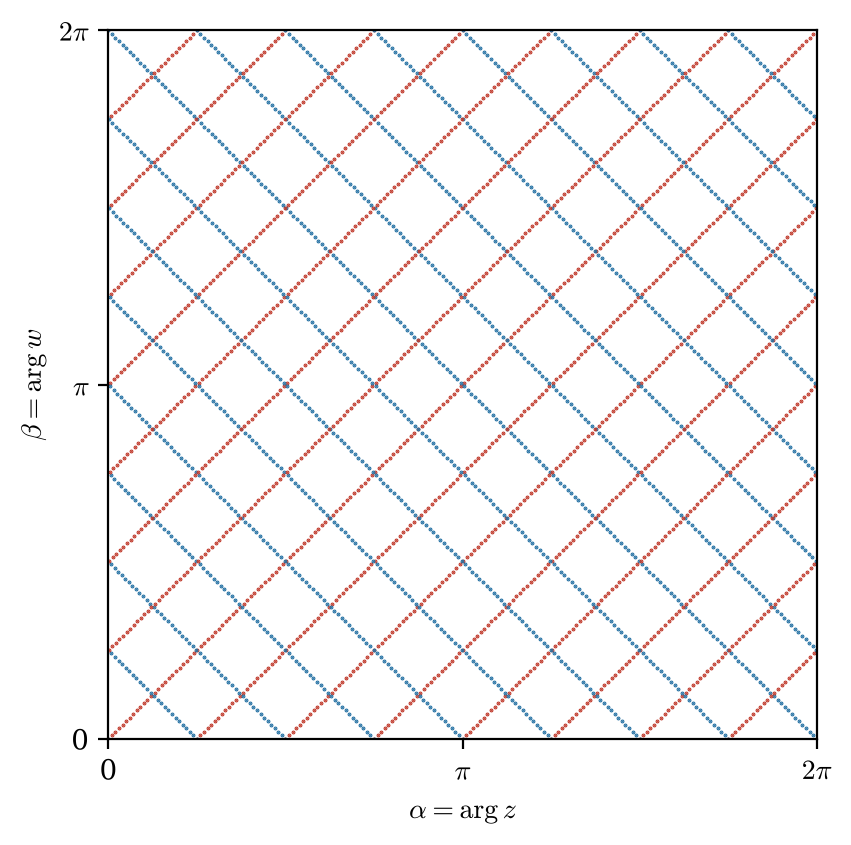
\includegraphics[width=0.9\textwidth]{fig_clifford.png}
\caption{The flat torus $T_{a,b}$ unrolled in arc-length coordinates, for $a=0.6$, $b=0.8$. The Hopf fibres are the lines of slope $b/a$ (solid), and the fibres of $(z,w)\mapsto h(\bar z,w)$ are the lines of slope $-b/a$ (dashed). After stereographic projection the two families become the two families of Villarceau circles (Chapter~\ref{ch:villarceau}).}
\label{fig:clifford}
\end{figure}

\begin{figure}[ht]
\centering
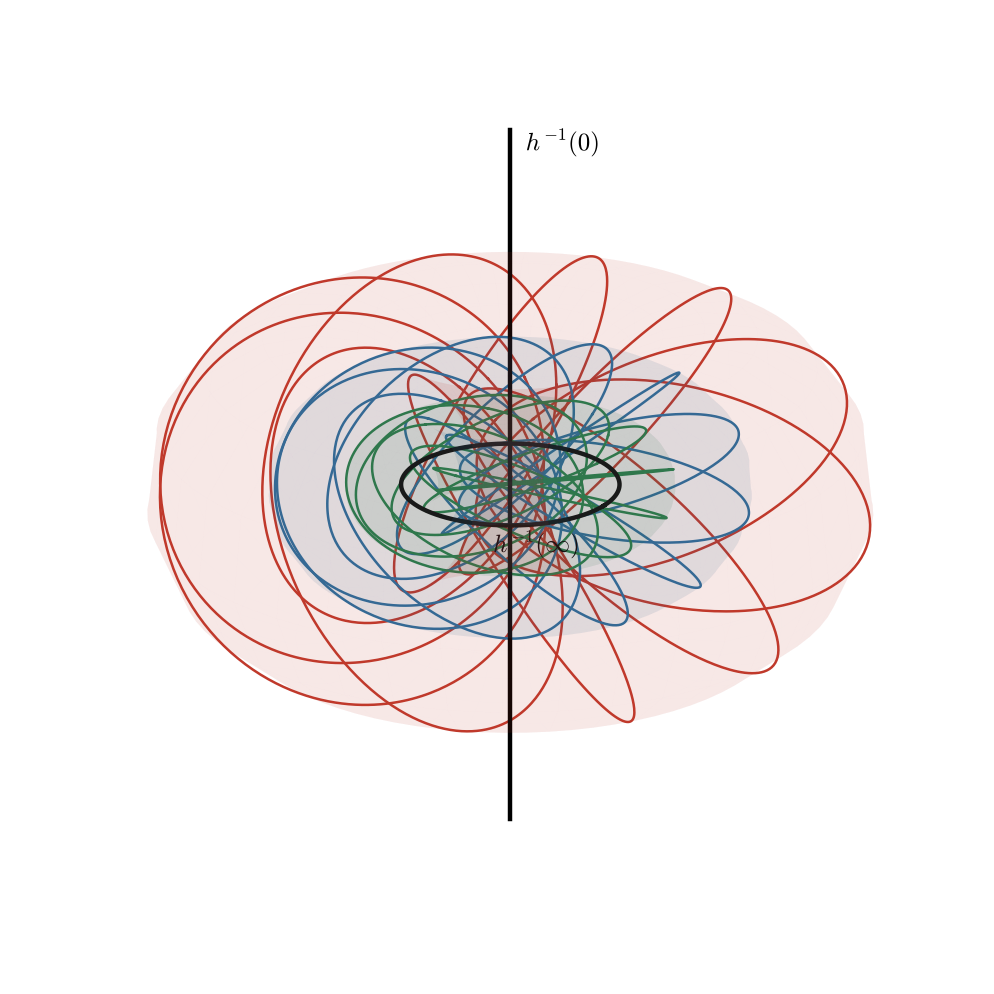
\includegraphics[width=0.85\textwidth]{fig_hopf_tori.png}
\caption{Nested tori $T_{a,b}$ in $\R^3$ after stereographic projection, each with some of its Hopf fibres; the vertical axis together with $\infty$ is the fibre over one pole, and the unit circle in the horizontal plane is the fibre over the other.}
\label{fig:hopftori}
\end{figure}

\section{The unit tangent bundle of the two-sphere}\label{sec:unittangent}

Identify $\R^3$ with $\Imag\Hq$ and $S^3$ with the unit quaternions. The map $\rho(q)(v)=qv\bar q$ is a surjective homomorphism $S^3\to\SO(3)$ with kernel $\{\pm1\}$ \cite[Section~2.3]{Bae02}, so $\SO(3)\cong S^3/\{\pm1\}=\RP^3$.

\begin{proposition}\label{prop:unittangent}
Let $T^1S^2=\{(p,v)\in S^2\times S^2:p\perp v\}$ be the unit tangent bundle. The map $\Psi\colon S^3\to T^1S^2$, $\Psi(q)=(qi\bar q,\,qj\bar q)$, is a two-fold covering that identifies $T^1S^2$ with $\RP^3$. Its composite with the projection to $S^2$ is $h'(q)=qi\bar q$, which is the Hopf map up to isometries of $S^3$ and of $S^2$, and the circle bundle $T^1S^2\to S^2$ is the quotient of the Hopf bundle by the antipodal action $q\mapsto-q$ on its fibres.
\end{proposition}

\begin{proof}
A point $(p,v)$ of $T^1S^2$ determines the positive orthonormal frame $(p,v,p\times v)$, and $\SO(3)$ acts simply transitively on such frames, so $(p,v)\mapsto$ the rotation taking $(i,j,k)$ to the frame is a diffeomorphism $T^1S^2\cong\SO(3)$, and $\Psi$ corresponds to $\rho$. For $q=z+wj$ with $z,w\in\C$ a direct computation, using $ji=-ij$ and $wj=j\bar w$, gives
\[
qi\bar q=(|z|^2-|w|^2)\,i+2\Imag(zw)\,j-2\Re(zw)\,k,
\]
which is $h(z,\bar w)=(2zw,|z|^2-|w|^2)$ followed by a linear isometry of $\R^3$. The fibres of $h'$ are the circles $\{qe^{i\theta}\}$, and $\Psi(qe^{i\theta})=(qi\bar q,\,qe^{2i\theta}j\bar q)$, so as $\theta$ runs over $[0,\pi]$ the tangent vector turns once around $p=qi\bar q$; the points $q$ and $-q$ of a fibre of $h'$ give the same point of $T^1S^2$.
\end{proof}

\begin{remark}
The Euler number of the Hopf bundle is $\pm1$ and that of $T^1S^2\to S^2$ is $\chi(S^2)=2$, in accordance with the quotient by $\pm1$, which doubles the Euler class of an oriented circle bundle. The total space of $T^1S^2$ is $\RP^3$, not $S^3$; its fundamental group is $\Z/2$, while $S^3$ is simply connected. Theorem~\ref{thm:F} follows from Propositions~\ref{prop:parallel}, \ref{prop:clifford} and \ref{prop:unittangent}.
\end{remark}
